\section{Simple tuning of hand-built grammar with curves of constant length}

Here is our example curve, from which we build a grammar with
hand-chosen rules. It is the grammar shown in section 1.

\begin{figure}
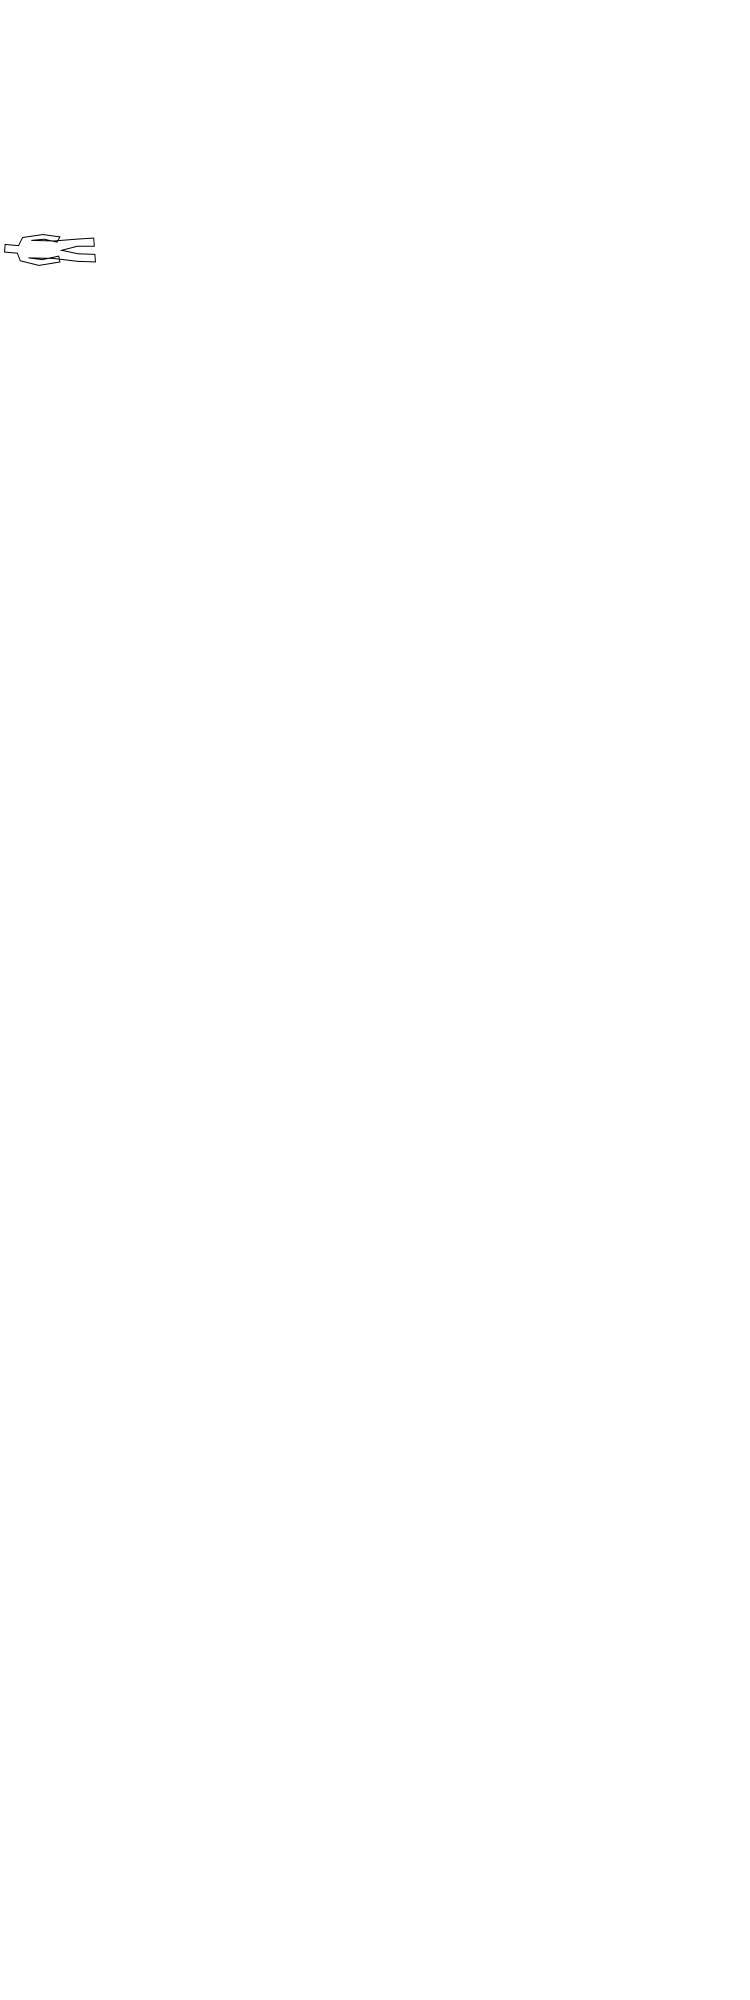
\includegraphics[width=\linewidth]{experiments/3.em/simple_tuning/output.d/examples.png}
\caption{Here is our example curve, from which we build a grammar with hand-chosen rules.}
\end{figure}

Here are our training curves:

\begin{figure}
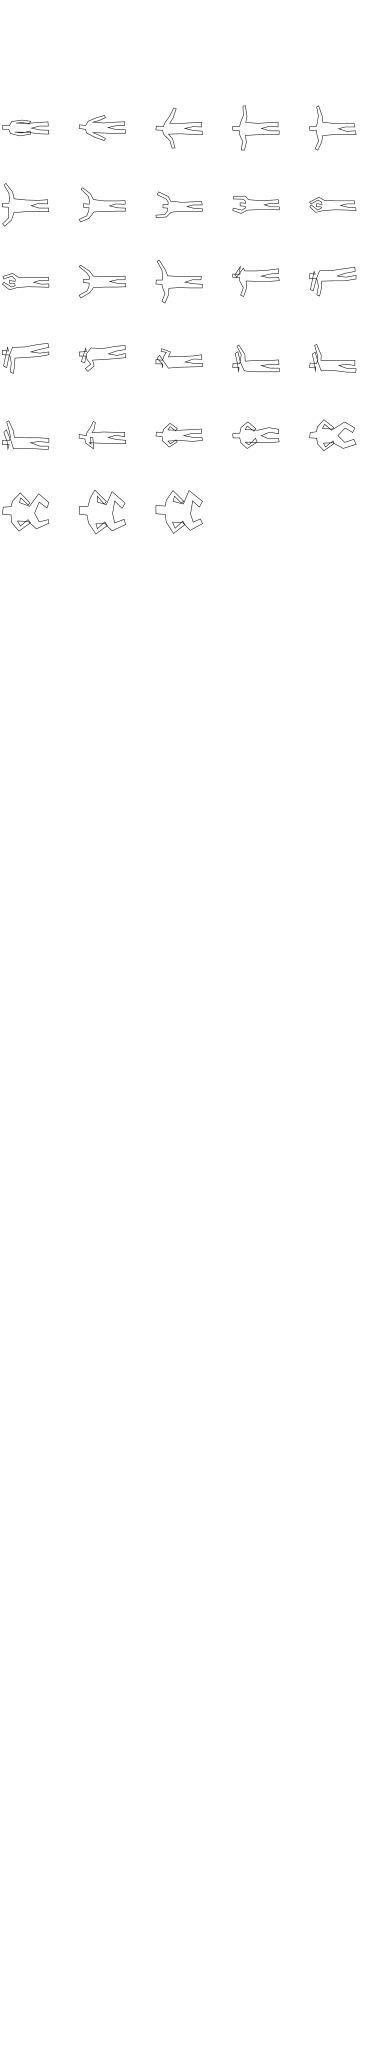
\includegraphics[width=4in]{experiments/3.em/simple_tuning/output.d/training.png}
\caption{Here are our training curves:}
\end{figure}

Round 2:

Here are some samples from the grammar:

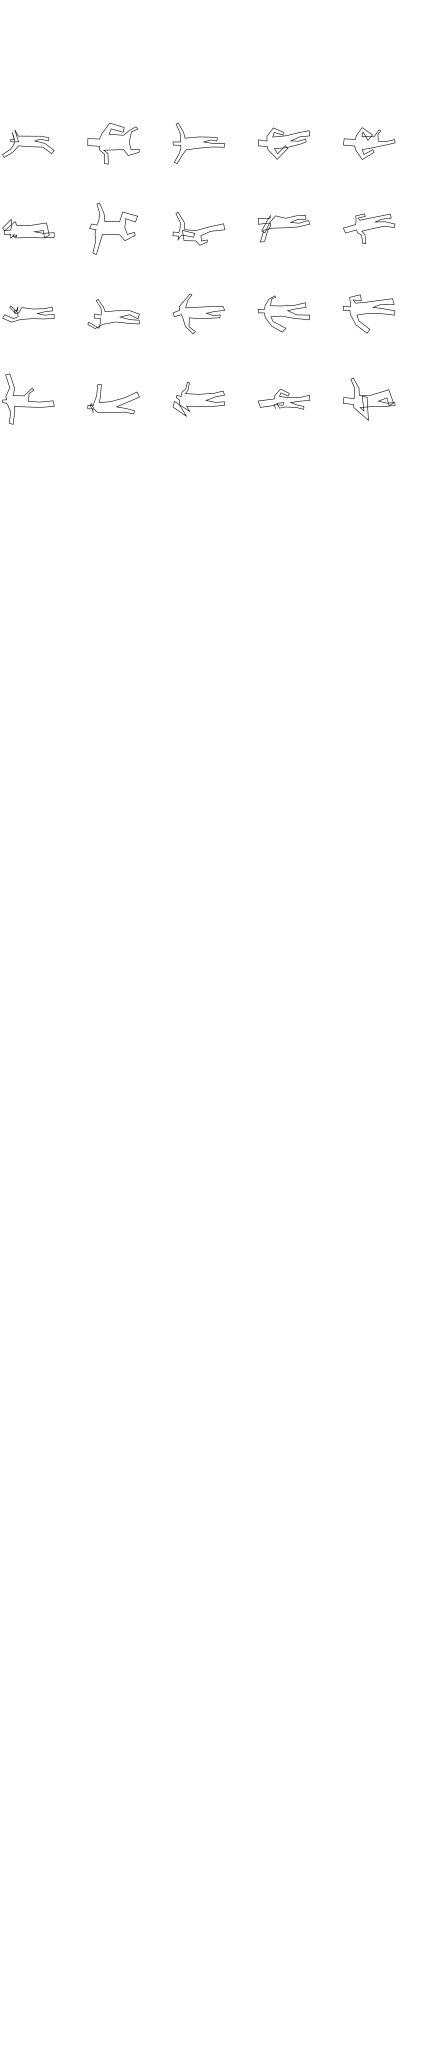
\includegraphics[width=6in]{output/3.learning/incremental/gram.30.d/samples.png}


